\subsection{IPS algortihm for modified Merton's Model}
The following parameters were used across experiments and observations were made
on these:
\begin{center}
	\begin{tabular}{|c|c|}
		\hline
		Parameter       & Value                              \\
		\hline
		\multicolumn{2}{|c|}{\textbf{General Parameters}}\\
		\hline
		N               & 125                                \\
		\hline
		M               & 20 - 2000                          \\
		\hline
		$\alpha $       & 0.05 - 0.5 (100 values in between) \\
		\hline
		T               & $1, 2, 3, 4, 5$                    \\
		\hline
		\multicolumn{2}{|c|}{\textbf{Stochastic Volatility Parameters} (Equation
		\ref{eq:merton_volatility_sde})}\\
		\hline
		$\sigma$(0)     & 0.4                                \\
		\hline
		$\kappa $       & 3.5                                \\
		\hline
		$\bar{\sigma}$  & 0.4                                \\
		\hline
		$\gamma$        & 0.7                                \\
		\hline
		$\rho_{\sigma}$ & -0.06                              \\
		\hline
		\multicolumn{2}{|c|}{\textbf{Asset Parameters} (Equation \ref{eq:merton_asset_sde})}\\
		\hline
		$S_i(0)$        & 90                                 \\
		\hline
		r               & 0.06                               \\
		\hline
		$\rho$          & 0.1                                \\
		\hline
		$B_i$           & 36                                 \\
		\hline
		$N_{sel}$       & 20                                 \\
		\hline
		$\delta t$      & $10^{-3}$                          \\
		\hline
	\end{tabular}
\end{center}

For the sake of simplistic simulations we take the starting point, barrier
level, correlation structure of all assets to be the same.

Figure \ref{fig:IPS_all} shows the probability distribution of the number of
loss L(T) for $T = 1, 2, 3, 4$. We see that we have managed to obtain the
probability for large number of defaults with only a few number of samples ($M =
200/2000$). Also as we would expect the probability of larger defaults increases
as the simulated maturity period increases.

In Figure \ref{fig:IPS_comparison}, we see the effect of number of samples
taken. The point to observe here is that given enough values of $\alpha$, 
increasing $M$ from 200 to 2000 does not drastically affect the generated
probabilities. This speaks to the efficiency of the algorithm in selecting
appropriate paths to simulate rare events.

Another point of note is that we run $100$ IPS runs with values of $\alpha$
equally spaced between $0.05$ to $0.5$ and choose the best $\alpha$ for a given
range of defaults as suggested in \cite{carmona2009importance}. The reason for 
doing so is because for a given value of $\alpha$, the IPS algorithm is able to 
estimate $\mathbb{P}(L(T) = k)$ without bias only for some values of $k$. This
is a well studied fact as the IPS algortihm tends to concentrate on a small set
of paths. This effect is clearly seen in Figure \ref{fig:IPS_surface}.

\subsubsection{Single Asset Constant Volatility Case}
We proceed with the analysis of a single asset constant volatility as it can be
compared against known solution of a default over a maturity period $T$. For
this we used a constant volatility of $0.25$ and $\alpha = 18.5$.

We then use the analytically derived default probabilities from Section
\ref{subsubsec:single_asset} to compare against our estimated probabilites to
show how good these estimates are.

As shown in Figure \ref{fig:IPS_single},  we can see that the IPS algorithm
accurately estimates the default probabilities for a good range of
$\text{barrier}/S_0$ value. It even manages to trace default probabilities of the 
order of $10^{-14}$ which is quite remarkable. This indicates that the IPS
algorithm is quite effective in sampling these rare events and is doing so quite
accurately. In the same figure we can see that the MC algorithm is unable to
estimate low probability defaults just as expected.

\begin{figure}
	\centering
	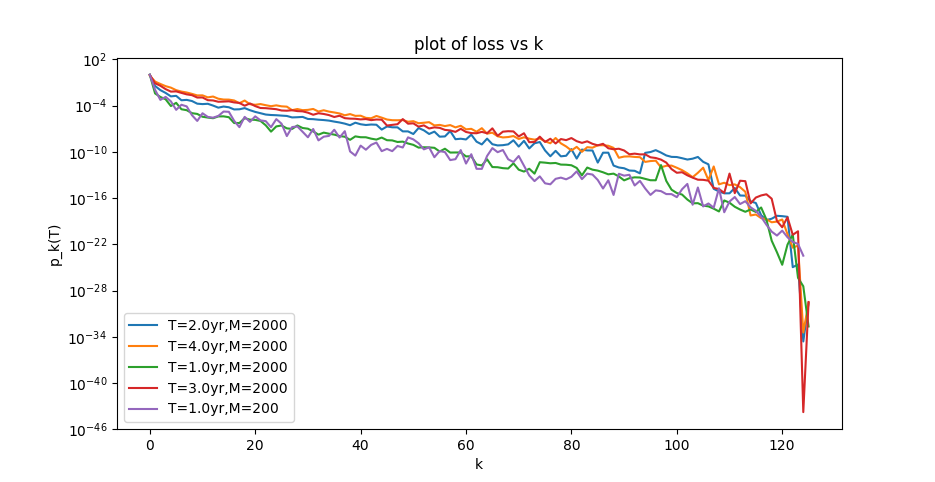
\includegraphics[width=\textwidth]{IPS_all_years}
	\caption{Plot of default probabilities for each level and maturity times
	based on IPS}
	\label{fig:IPS_all}
\end{figure}

\begin{figure}
	\centering
	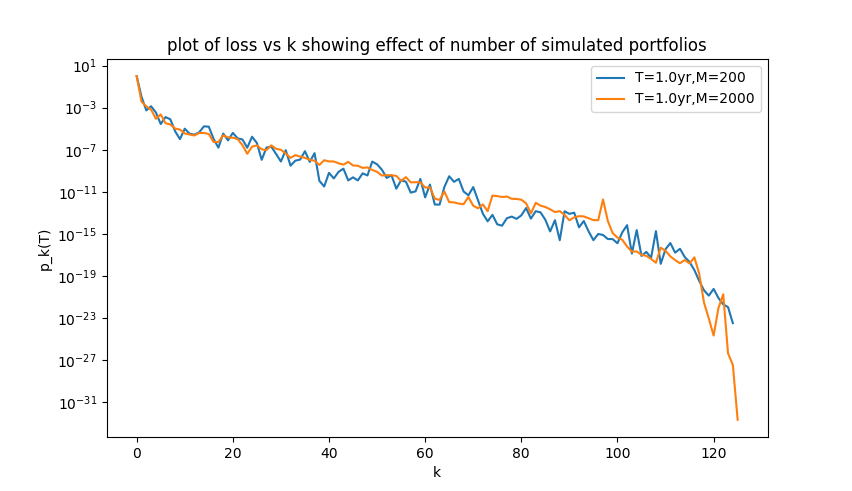
\includegraphics[width=\textwidth]{IPS_M_comparison}
	\caption{Plot comparing default probabilities for maturity $T=1$ with
	different number of portfolios}
	\label{fig:IPS_comparison}
\end{figure}

\begin{figure}
	\centering
	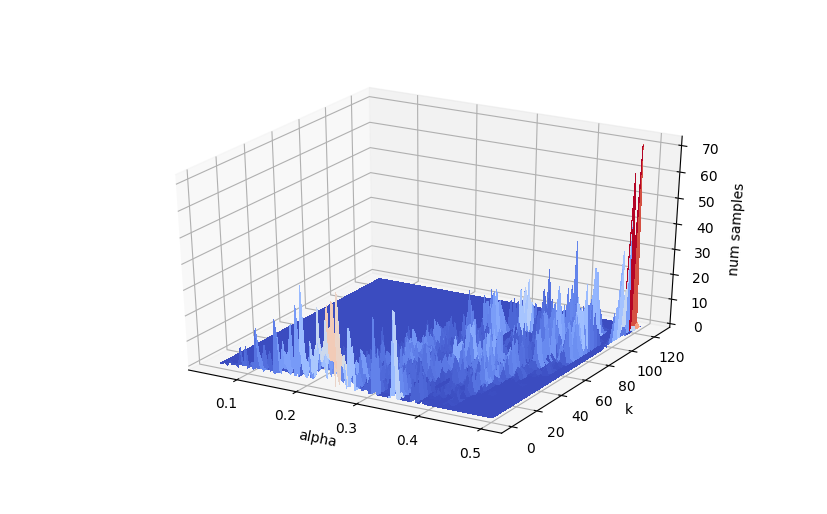
\includegraphics[width = \textwidth]{IPS_surface}
	\caption{Plot of number of defaults simulated for $\alpha$, $k$ combination}
	\label{fig:IPS_surface}
\end{figure}

\begin{figure}
	\centering
	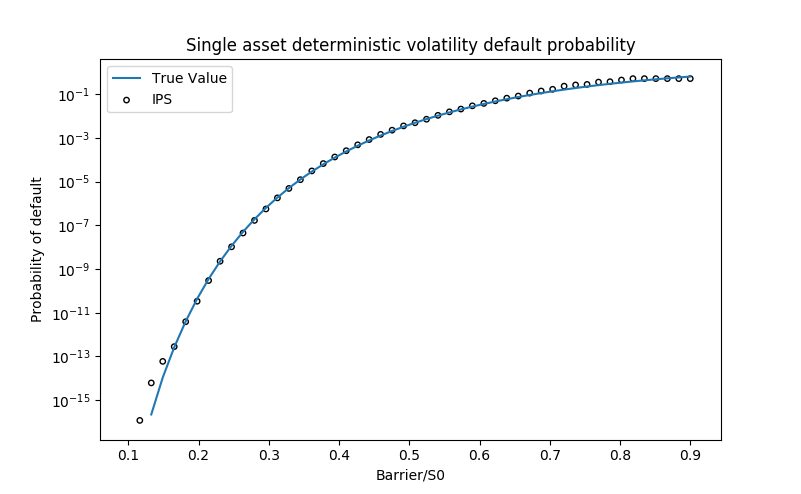
\includegraphics[width = \textwidth]{IPS_single}
	\caption{Default probabilities of different barrier levels for single asset
	deterministic volatility case}
	\label{fig:IPS_single}
\end{figure}
